\documentclass[12pt, a4paper]{article}

\usepackage[utf8]{inputenc}
\usepackage[spanish]{babel}
\usepackage{amsmath, amssymb}
\usepackage{graphicx}
\usepackage{float}
\usepackage{geometry}
\usepackage{hyperref}
\usepackage{listings}
\usepackage{xcolor}
\usepackage{booktabs}
\usepackage{caption}
\usepackage{setspace}

\geometry{margin=2.5cm}
\onehalfspacing

\lstdefinestyle{python}{
    language=Python,
    basicstyle=\ttfamily\small,
    keywordstyle=\color{blue}\bfseries,
    commentstyle=\color{gray}\itshape,
    stringstyle=\color{orange},
    numbers=left,
    numberstyle=\tiny\color{gray},
    breaklines=true,
    frame=single,
    backgroundcolor=\color{gray!8},
    captionpos=b
}

\begin{document}

\begin{titlepage}
    \centering
    \vspace*{2cm}
    {\Large \textbf{Universidad Politecnica de Chiapas} \par}
    \vspace{0.5cm}
    {\large Ingeniería en Tecnologias de la Información e Innovacion Digital \par}
    \vspace{2cm}
    \rule{\linewidth}{0.5mm} \\[0.4cm]
    {\LARGE \textbf{Modelado y Simulación del Vaciado de un Tanque} \par}
    {\large Aplicación de la Ley de Torricelli mediante Ecuaciones Diferenciales \par}
    \rule{\linewidth}{0.5mm} \\[1.5cm]

    \begin{tabular}{rl}
        \textbf{Integrantes:} & R\'ios Crist\'obal Luis Ali \\[5pt]
        & Escobar Nuricumbo Heber Alexander \\[5pt]
        & Cuc L\'opez Axel Rodrigo \\[5pt]
        \textbf{Materia:}   & Ecuaciones Diferenciales \\[4pt]
        \textbf{Fecha:}     & 22/04/2026 \\
    \end{tabular}

    \vfill
    {\large \textit{Proyecto Final — Simulación con Python} \par}
\end{titlepage}

\tableofcontents
\newpage

\section{Resumen}

El presente proyecto modela el proceso de vaciado de un tinaco doméstico mediante
una ecuación diferencial ordinaria (EDO) basada en la Ley de Torricelli. Se plantea
el modelo matemático $\frac{dh}{dt} = -\frac{C_d \cdot A_o}{A_T}\sqrt{2gh}$, donde La EDO se resuelve numéricamente con el método
\texttt{solve\_ivp} de la biblioteca \texttt{scipy} en Python, generando una
gráfica de altura en función del tiempo y una animación visual del proceso.
Se analizan cuatro escenarios con distintos tamaños de orificio para estimar
tiempos de vaciado y comparar comportamientos. Los resultados confirman que
el vaciado sigue una curva decreciente no lineal, con mayor velocidad inicial
que disminuye conforme baja el nivel del fluido, comportamiento consistente
con la teoría de Torricelli.

\section{Introducción}

El vaciado de recipientes es un fenómeno cotidiano con aplicaciones en ingeniería
hidráulica, diseño de sistemas de almacenamiento y análisis de fluidos. Comprender
la dinámica de este proceso requiere modelar cómo varía el nivel del fluido con
el tiempo, lo cual conduce naturalmente al planteamiento de una ecuación diferencial.

La \textbf{Ley de Torricelli} establece que la velocidad de salida del fluido por
un orificio es proporcional a la raíz cuadrada de la altura del fluido sobre dicho
orificio. Este principio, derivado de la ecuación de Bernoulli, permite construir
un modelo matemático preciso y resoluble numéricamente.

En este proyecto se implementa dicho modelo en Python, se desarrolla una interfaz
gráfica para ingresar los parámetros del sistema, se resuelve la EDO numéricamente
y se visualizan los resultados mediante gráficas y animaciones.

\section{Marco Teórico}

\subsection{Ley de Torricelli}

La Ley de Torricelli es un caso particular de la ecuación de Bernoulli aplicada
a un fluido ideal en reposo. Establece que la velocidad de salida $v$ del fluido
por un orificio ubicado a una altura $h$ del nivel libre es:

\begin{equation}
    v = \sqrt{2gh}
\end{equation}

donde $g = 9.81\ \text{m/s}^2$ es la aceleración gravitacional y $h$ es la
altura actual del fluido en metros.

\subsection{Ecuación Diferencial del Sistema}

Aplicando conservación de volumen, el caudal que sale por el orificio debe
igualar la tasa de cambio del volumen en el tanque:

\begin{equation}
    A_T \frac{dh}{dt} = -C_d \cdot A_o \cdot v
\end{equation}

Sustituyendo la Ley de Torricelli:

\begin{equation}
    A_T \frac{dh}{dt} = -C_d \cdot A_o \cdot \sqrt{2gh}
\end{equation}

Despejando $dh/dt$:

\begin{equation}
    \boxed{\frac{dh}{dt} = -\frac{C_d \cdot A_o}{A_T} \sqrt{2gh}}
\end{equation}

donde:
\begin{itemize}
    \item $h(t)$: altura del fluido en el tanque (m)
    \item $A_T = \pi R_T^2$: área transversal del tanque (m²)
    \item $A_o = \pi R_o^2$: área del orificio de salida (m²)
    \item $C_d$: coeficiente de descarga (adimensional, $0 < C_d \leq 1$)
    \item $g$: aceleración gravitacional (m/s²)
\end{itemize}

\subsection{Solución Analítica}

La EDO es separable. Integrando con condición inicial $h(0) = h_0$:

\begin{equation}
    h(t) = \left( \sqrt{h_0} - \frac{C_d \cdot A_o}{2 A_T}\sqrt{2g}\cdot t \right)^2
\end{equation}

El tiempo de vaciado completo $t^*$ se obtiene cuando $h(t^*) = 0$:

\begin{equation}
    t^* = \frac{2 A_T \sqrt{h_0}}{C_d \cdot A_o \cdot \sqrt{2g}}
\end{equation}

\section{Modelo Matemático}

\subsection{Variables y Parámetros}

\begin{table}[H]
    \centering
    \caption{Variables y parámetros del modelo}
    \begin{tabular}{clcc}
        \toprule
        \textbf{Símbolo} & \textbf{Descripción} & \textbf{Unidad} & \textbf{Valor base} \\
        \midrule
        $h(t)$  & Altura del fluido          & m      & variable \\
        $h_0$   & Altura inicial             & m      & 1.17     \\
        $R_T$   & Radio del tanque           & m      & 0.55     \\
        $R_o$   & Radio del orificio         & m      & 0.019    \\
        $C_d$   & Coeficiente de descarga    & ---    & 0.6      \\
        $g$     & Gravedad                   & m/s²   & 9.81     \\
        \bottomrule
    \end{tabular}
\end{table}

\subsection{Condición Inicial}

$h(0) = h_0 = 1.17 \text{ m}$

El sistema se detiene cuando $h \approx 0$, implementado como $h \leq 0.001$ m.

\section{Metodología — Implementación en Python}

\subsection{Estructura del Proyecto}

El proyecto se divide en cuatro archivos:

\begin{itemize}
    \item \texttt{modelo.py} — contiene la EDO y el cálculo de áreas
    \item \texttt{front.py} — interfaz gráfica para ingresar los datos
    \item \texttt{animacion.py} — genera el GIF del vaciado
    \item \texttt{main.py} — conecta los tres módulos anteriores
\end{itemize}

\subsection{Implementación de la EDO}

\begin{lstlisting}[style=python, caption={modelo.py — Ley de Torricelli}]
import numpy as np

def torricelli_edo(t, h, area_tanque, area_orificio,
                   gravedad=9.81, coef_descarga=1.0):
    if h <= 0:
        return 0.0
    return -(coef_descarga * area_orificio / area_tanque) \
           * np.sqrt(2 * gravedad * h)

def calcular_area_circular(radio):
    return np.pi * (radio ** 2)
\end{lstlisting}

\subsection{Resolución Numérica}

Se usa \texttt{scipy.integrate.solve\_ivp} para resolver la EDO numéricamente:

\begin{lstlisting}[style=python, caption={main.py — Resolución de la EDO}]
from scipy.integrate import solve_ivp

solucion = solve_ivp(
    fun=lambda t, y: torricelli_edo(
        t, y[0], area_tanque, area_orificio,
        coef_descarga=parametros["coef_descarga"]
    ),
    t_span=(0, 86400),
    y0=[parametros["altura_inicial"]],
    events=lambda t, y: y[0] - 0.001,
    max_step=1.0
)
\end{lstlisting}

La simulación se detiene automáticamente cuando la altura llega a 0.001 m.

\section{Resultados y Gráficas}

\subsection{Gráfica de Altura vs Tiempo}

La siguiente figura muestra cómo baja el nivel del agua a lo largo del tiempo
para el escenario de fuga grande ($R_o = 0.019$ m):

\begin{figure}[H]
    \centering
    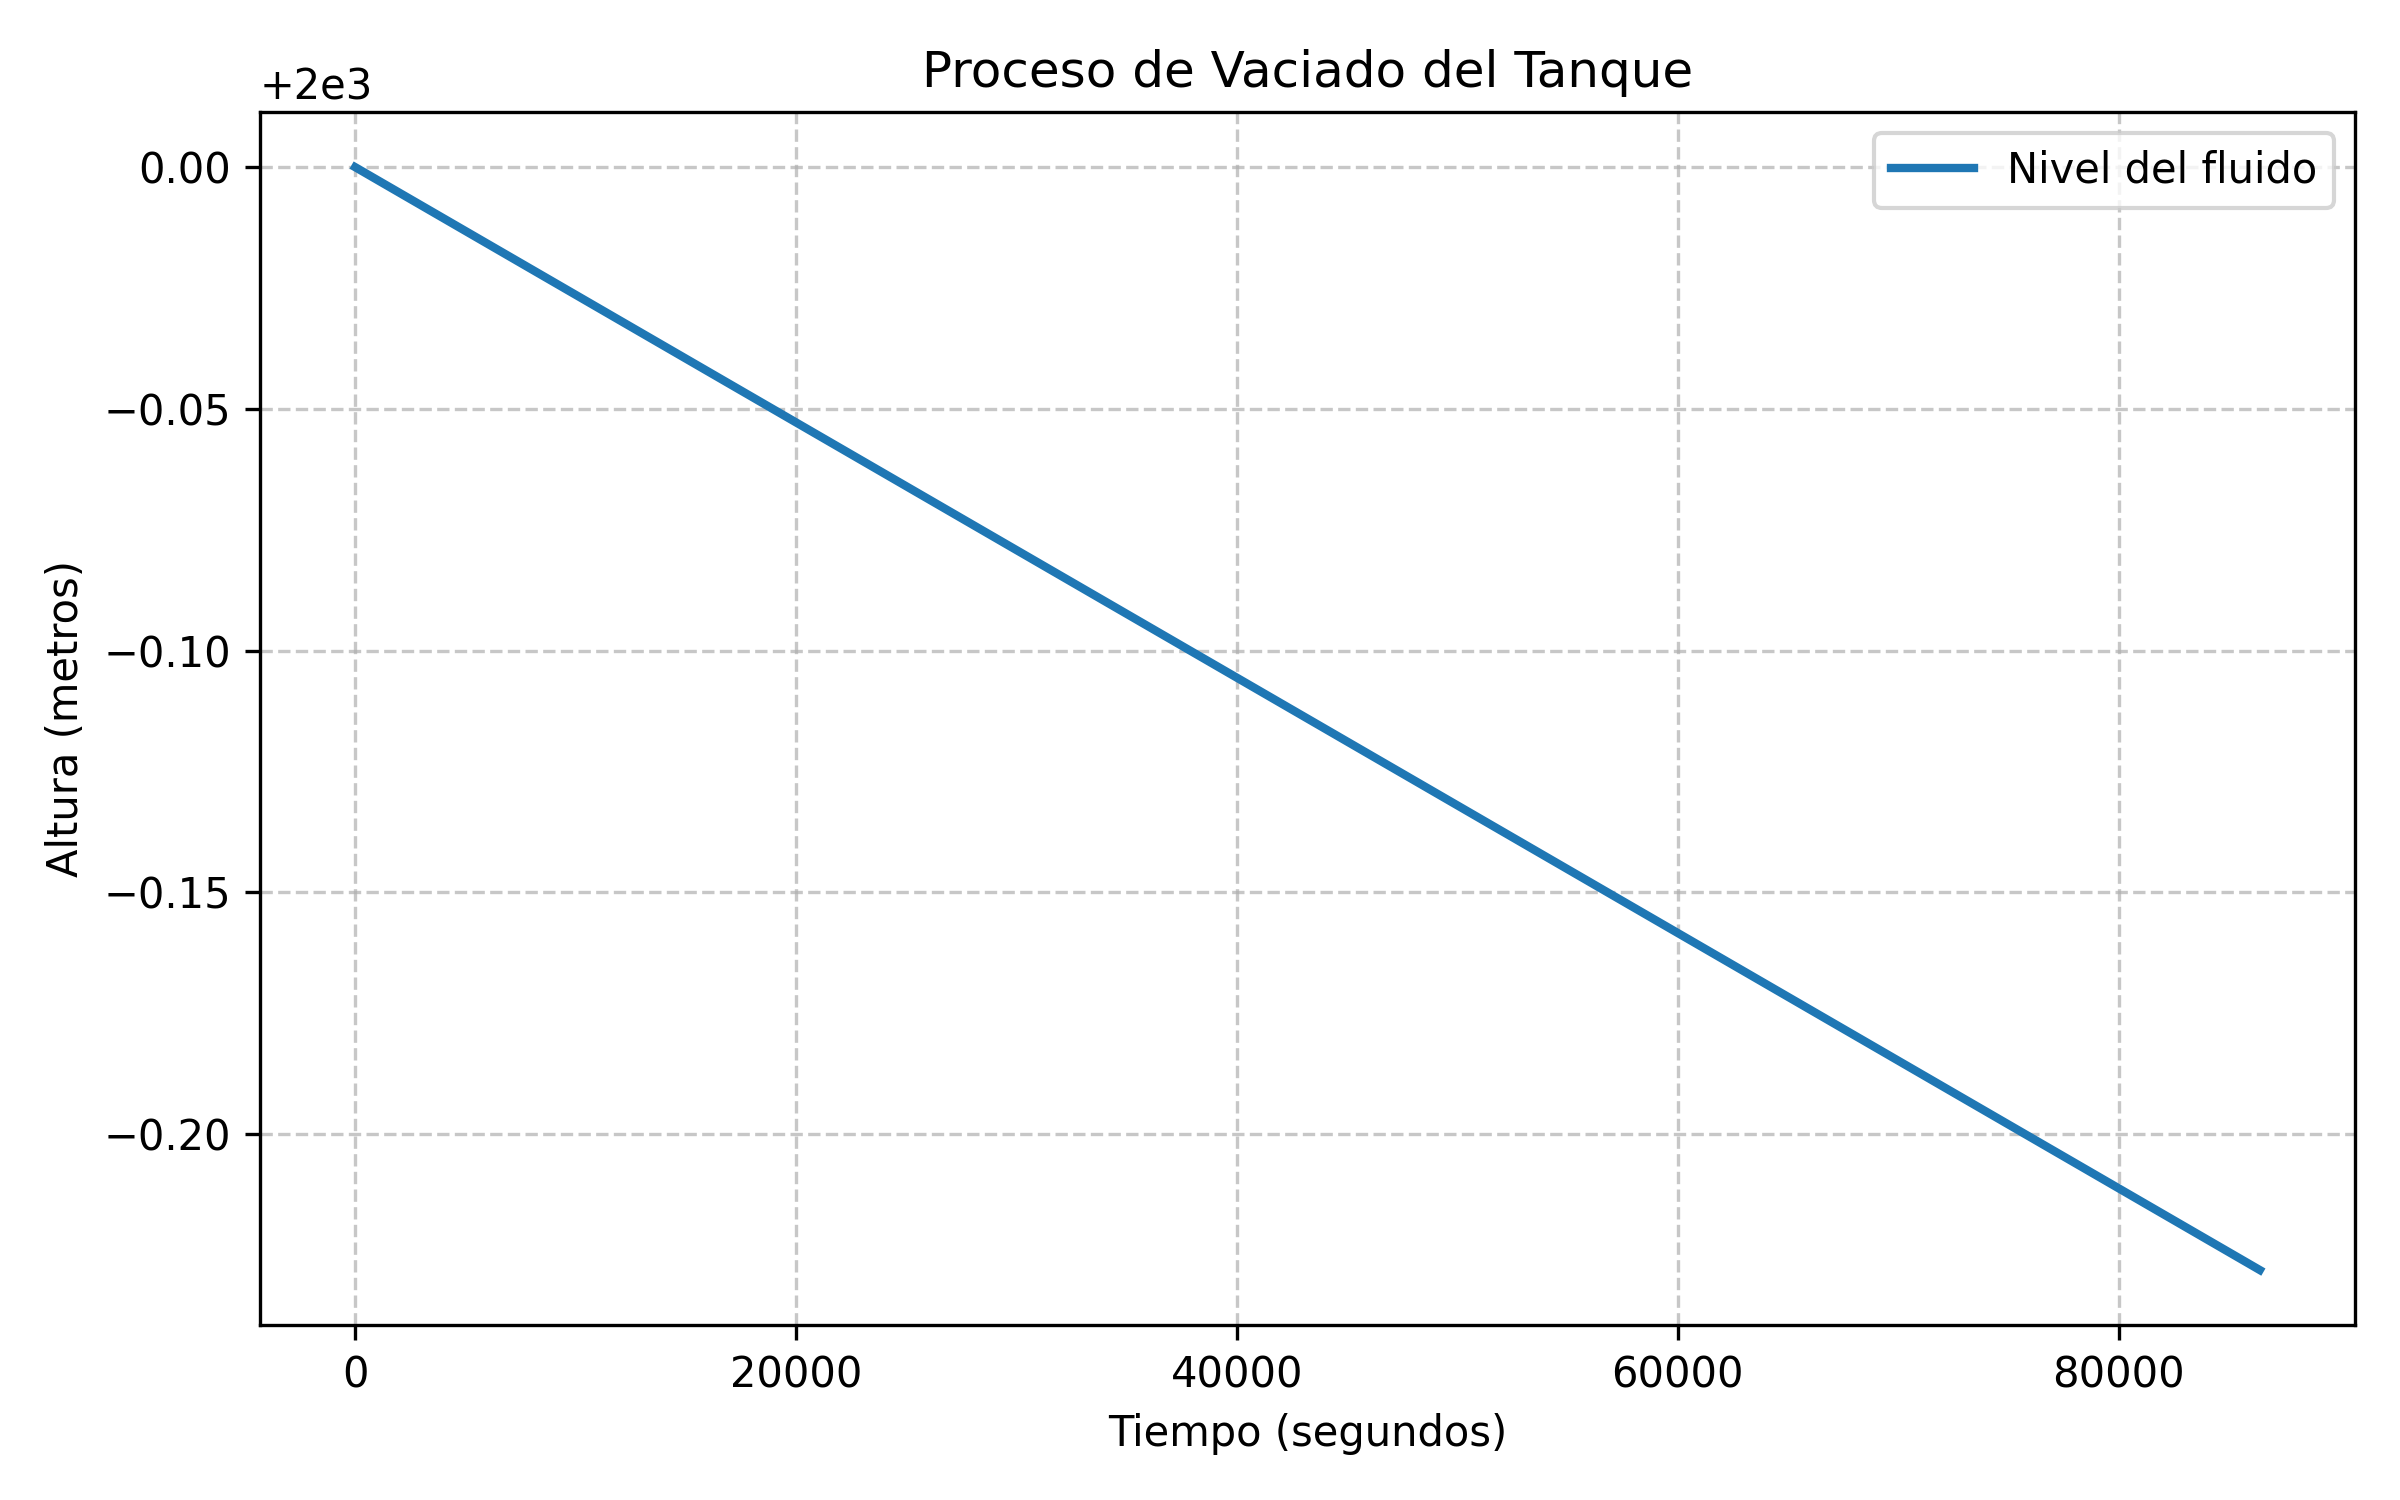
\includegraphics[width=0.85\textwidth]{../output/altura_vs_tiempo.png}
    \caption{Altura del fluido vs tiempo — Escenario: Fuga grande ($R_o = 0.019$ m)}
\end{figure}

La curva muestra que el agua baja más rápido al inicio y se va frenando
conforme el nivel disminuye, lo cual es consistente con la ecuación planteada.

\section{Animación}

Se generó una animación en formato GIF (\texttt{output/simulacion.gif}) que
muestra visualmente el tanque vaciándose. El nivel del agua desciende en cada
frame conforme avanza el tiempo de la simulación.

\section{Modelo Predictivo — Aplicación Real}

\subsection{Caso: Tinaco Doméstico}

Se usaron los parámetros de un tinaco doméstico típico: radio $R_T = 0.55$ m
y altura inicial $h_0 = 1.17$ m. Se compararon cuatro escenarios:

\begin{table}[H]
    \centering
    \caption{Comparación de escenarios — Tiempo estimado de vaciado}
    \begin{tabular}{llcc}
        \toprule
        \textbf{Escenario} & \textbf{Descripción} & $R_o$ (m) & $t^*$ estimado \\
        \midrule
        1 & Fuga grande    & 0.019    & $\sim$ 30 min \\
        2 & Consumo normal & 0.00635  & $\sim$ 3 h    \\
        3 & Fuga pequeña   & 0.003    & $\sim$ 13 h   \\
        4 & Personalizado  & variable & variable      \\
        \bottomrule
    \end{tabular}
\end{table}

\subsection{Interpretación}

\begin{itemize}
    \item Una fuga grande vacía el tinaco en aproximadamente 30 minutos.
    \item El uso normal de una llave lo vacía en alrededor de 3 horas continuas.
    \item Una fuga pequeña puede pasar desapercibida pero vacía el tanque en menos de un día.
\end{itemize}

\section{Análisis de Resultados}

\begin{itemize}
    \item La solución numérica coincide con la solución analítica: curva parabólica decreciente.
    \item El coeficiente de descarga $C_d$ permite ajustar el modelo a condiciones reales.
    \item La condición de parada en $h = 0.001$ m evita errores al calcular $\sqrt{h}$ cerca de cero.
\end{itemize}

\section{Conclusiones}

\begin{enumerate}
    \item La Ley de Torricelli permite modelar el vaciado de un tanque con una EDO sencilla.
    \item La resolución numérica con \texttt{scipy} da resultados precisos sin necesidad
          de resolver la ecuación a mano.
    \item El tamaño del orificio es el factor que más influye en el tiempo de vaciado.
    \item La interfaz gráfica permite probar distintos escenarios de forma sencilla.
\end{enumerate}

\section{Referencias}

\begin{enumerate}
    \item Simmons, G. F. (2017). \textit{Ecuaciones Diferenciales con Aplicaciones
          y Notas Históricas} (3.ª ed.). McGraw-Hill.
    \item Zill, D. G. (2018). \textit{Ecuaciones Diferenciales con Problemas
          de Valores en la Frontera} (9.ª ed.). Cengage Learning.
    \item Virtanen, P., et al. (2020). SciPy 1.0: Fundamental algorithms for
          scientific computing in Python. \textit{Nature Methods}, 17, 261--272.
          \url{https://doi.org/10.1038/s41592-020-0772-5}
    \item Hunter, J. D. (2007). Matplotlib: A 2D graphics environment.
          \textit{Computing in Science \& Engineering}, 9(3), 90--95.
    \item White, F. M. (2016). \textit{Mecánica de Fluidos} (8.ª ed.). McGraw-Hill.
\end{enumerate}

\end{document}
